\chapter{Reactive Programming}\label{chap:rp_reactive_programming} % (fold)
Both the \hyperref[def:cps]{CPS} and \hyperref[def:promises]{Promises} assume that asynchronous computations will deliver their result in \textit{one shot}.
However, it's not uncommon in application the need to manage \textbf{asynchronous streams} of data/events; this is the goal of \textbf{Reactive Programming} (asynchronous data stream programming).
\emptyln{}
The reactive programming paradigm is oriented around \textbf{data flows} and the propagation of change, easing the management of asynchronous streams of data and events: strongly related to the \textbf{Observer pattern} \& \hyperref[sec:rs_event_driven_programming]{Event-Driven Programming}.
\begin{note}[\ac{frp}]
    Based on the \textit{synchronous data flow programming} paradigm but with relaxed real-time constraints
\end{note}
Asynchronous programs and applications are difficult to program using conventional sequential programming approaches, because it is impossible to predict or control the order of arrival of external events.
\begin{note}
    Control jumps around event handlers as the outside environment changes unexpectedly
\end{note}
The \textbf{Inversion of control} problem: the control flow of a program is driven by external events and not by an order specified by the programmer.
When there is a state change in one computation or data, the programmer is \textit{required to manually update all the others} that depend on it.
\begin{warning}
    Such manual management of state changes and data dependencies is complex and \textbf{error-prone}
\end{warning}
Coordinating callbacks can be a very daunting task even for advanced programmers: numerous isolated code fragments can be manipulating the same data and their order of execution is unpredictable.
\begin{critical}
    Since callbacks usually do not have a return value, they must perform \textit{side effects} in order to affect the application state
\end{critical}
\section{Reactive Programming Paradigm}\label{sec:rp_reactive_programming_paradigm} % (fold)
The RP paradigm provides abstractions to express programs as \textit{reactions} to external events.
But having the language automatically manage the flow of time, and data and computation dependencies: abstracting over time management, just as garbage collectors abstract over memory management.
\emptyln{}
RP facilitates the \textbf{declarative development of \hyperref[sec:rs_event_driven_programming]{Event-Driven}} applications:
\begin{itemize}
    \item developers can express programs in terms of what to do, and let the language automatically manage when to do it;
    \item built around the notion of \textbf{continuous time-varying values and propagation of change};
        \begin{note}
            State changes are automatically and efficiently propagated across the network of dependent computations by the underlying execution model
        \end{note}
\end{itemize}
\begin{example}{Change Propagation}{}
    Consider a simple example of calculating the sum of two variable:
    \begin{codeblock}[js]{}
    const var1 = 1;
    const var2 = 2;
    const var3 = var1 + var2;
    \end{codeblock}
    In reactive programming, the value of the variable \texttt{var3} is always kept up-to-date, the value is automatically recomputed over time whenever the value of \texttt{var1} or \texttt{var2} changes.
    \begin{note}
        Values change over time and when they change all dependent computations are automatically re-executed
    \end{note}
    In reactive programming terminology, the variable \texttt{var3} is said to be \textit{dependent} on the variables \texttt{var1} and \texttt{var2}.
\end{example}
%
\subsection{RP Abstractions}\label{sub:rp_rp_abstractions} % (fold)
Reactive programming abstracts \textit{time-varying events} for their consumption by a programmer, he can then define elements that will react upon each of these incoming time-varying events.
Abstractions are first-class values, and can be passed around or even composed within the program.
\emptyln{}
There are two main kinds of \textbf{reactive abstractions}:
\begin{itemize}
    \item \textbf{event streams}, modelling discrete or sparse time-varying values with asynchronous abstractions for the progressive flow of intermittent, sequential data coming from a recurring event (e.g. mouse events can be represented as event streams);
    \item \textbf{behaviours (or signals)}, continuous values over time where abstractions that represent uninterrupted fluid flow of incoming data from a steady event (e.g. a timer can be represented as a behaviour);
\end{itemize}
\begin{example}{A timer in Flapjax}{}
    \begin{codeblock}[js]{}
    var timer = timerB(100);
    var seconds = liftB(function (time) {
        return Math.floor(time / 1000);
    }, timer);
    insertDomB(seconds, "timer-div");
    \end{codeblock}
    This code block set up a DOM element in web page showing a timer count in seconds:
    \begin{itemize}
        \item first a timer behaviour producing a value after every $100$ milliseconds is created (\texttt{timer} is a behaviour variable);
        \item to show the time in second, a further behaviour variable is defined (\texttt{seconds)}, storing the flow in seconds;
        \item finally the \texttt{seconds} behaviour is inserted within the DOM element
    \end{itemize}
    \begin{note}
        Fully declarative way of managing events and event streams
    \end{note}
\end{example}
% subsection RP Abstractions (end)
%
\subsection{Evaluation Model}\label{sub:rp_evaluation_model} % (fold)
The evaluation model of a reactive programming language is concerned with ``\textit{how changes are propagated across a dependency graph of values and computations}''.
From the programmer's point of view, propagation of changes happens automatically:
\begin{itemize}
    \item a change of a value should be automatically propagated to all dependent computations;
    \item when there is an event occurrence at an event source, dependent computations need to be notified about the changes, possibly triggering a recomputation;
\end{itemize}
At the language level, the design decision that needs to be taken into account is who initiates the propagation of changes, whether:
\begin{itemize}
    \item the source should \textit{push} new data to its dependents (\textbf{consumers});
    \item the dependents should \textit{pull} data from the event source (\textbf{producer});
\end{itemize}
%
\subsubsection{Pull and Push Models}\label{sub:rp_pull_and_push_models} % (fold)
Two \hyperref[sub:rp_evaluation_model]{Evaluation Models}:
\begin{description}
    \item[Pull-based] The computation that requires a value needs to ``pull'' it from the source.
        The propagation is driven by the demand of new data (\textbf{demand-driven}), it can be implemented by lazy languages (e.g. Haskell).
    \item[Push-based] When the source has new data, it pushes the data to its dependent computations.
        The propagation is driven by availability of new data (\textbf{data-driven}), it's implemented by eager languages (e.g. Flapjax based on JavaScript, Scala, React).
\end{description}
% subsubsection Pull and Push Models (end)
%
\subsubsection{Glitches}\label{sub:rp_glitches} % (fold)
\textbf{Glitches} are update inconsistencies that may occur during the propagation of changes.
When a computation is run before all its dependent expressions are evaluated, it may result in fresh values being combined with stale values, leading to a glitch.
\begin{warning}
    Problem affecting only the \hyperref[sub:rp_pull_and_push_models]{Push-Based} evaluation model
\end{warning}
\begin{example}{}{}
    \begin{codeblock}[js]{}
    let var1 = 1;
    let var2 = var1 * 1;
    let var3 = var1 + var2;
    \end{codeblock}
    The value of the variable \texttt{var2} is expected to always be the same as that of \texttt{var1}, and \texttt{var3} to always be twice that of \texttt{var1}.
    When the value of \texttt{var1} is $1$, the value of \texttt{var2} is $1$ and \texttt{var3} is $2$.
    \begin{cimage}
        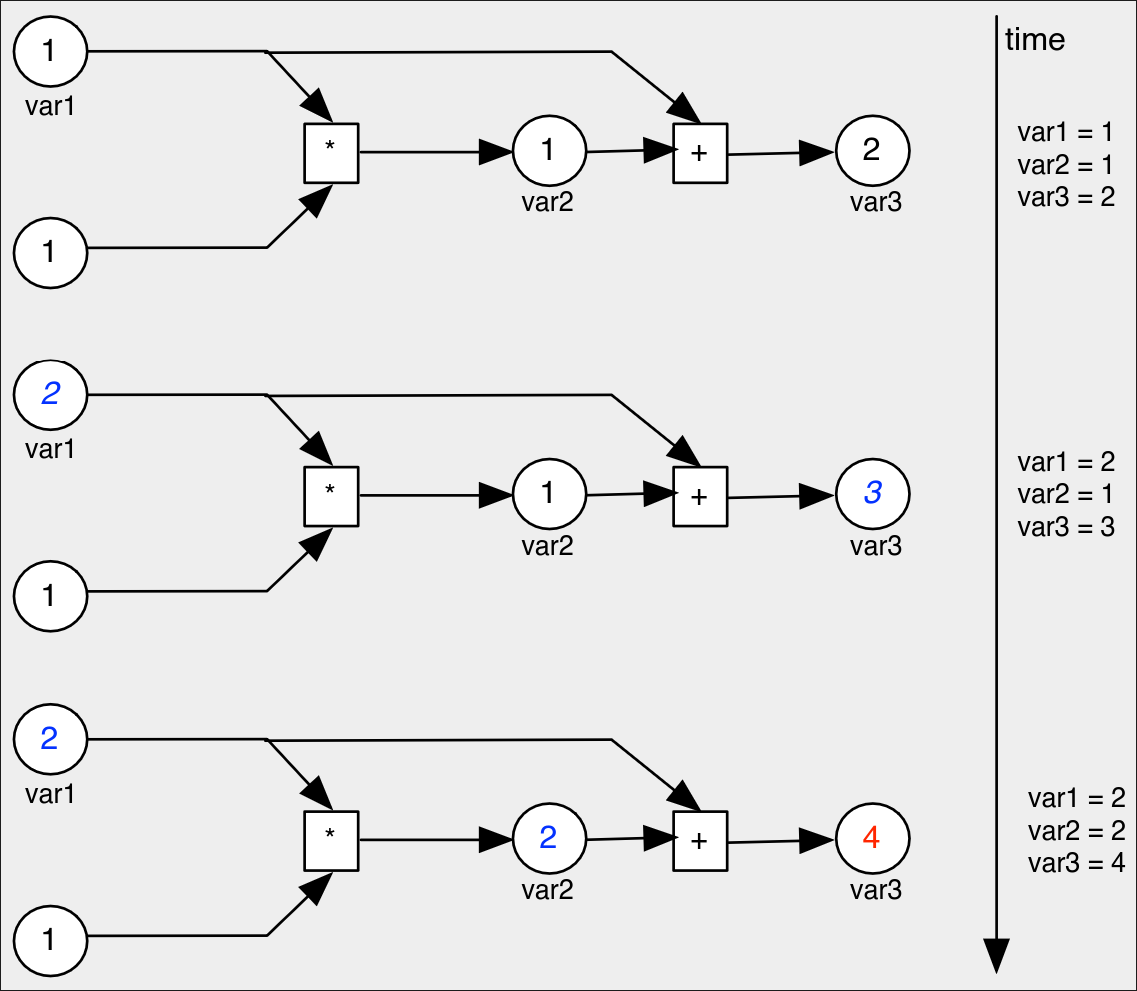
\includegraphics[width=.4\textwidth]{assets/20261124_101946.png}
    \end{cimage}
    If the value of \texttt{var1} changes to, say $2$, the value of \texttt{var2} is expected to change to $2$ while the value of \texttt{var3} is expected to be $4$.
    However, in a naive reactive implementation, changing the value of \texttt{var1} to $2$ may cause the expression \texttt{var1 + var2} to be recomputed before the expression \texttt{var1 * 1}.
    Thus, the value of \texttt{var3} will momentarily be $3$, which is incorrect.
    \emptyln{}
    Eventually, the expression \texttt{var1 * 1} will be recomputed to give a new value to \texttt{var2} and therefore the value of \texttt{var3} will be recomputed again to reflect the correct value $4$.
\end{example}
\begin{remark}{Glitch Avoidance}{}
    Most recent reactive implementations achieve glitch avoidance in reactive programs running on a single computer, but not in distributed reactive programs.
    Avoiding glitches in a distributing setting is not straightforward because of network failures, delay and lack of a global clock.
\end{remark}
% subsubsection Glitches (end)
% subsection Evaluation Model (end)
%
\subsection{Lifting}\label{sub:rp_lifting} % (fold)
The values in expressions that depend on the reactive values need to be reactive themselves.
A variable which gets assigned with some expression involving behaviours or event streams becomes a reactive variable itself, since updates from the behaviours/event streams will affect the variable itself.
\begin{definition}{Lifting}{lifting}
    The process of converting a normal variable into a reactive variable is called \textbf{lifting}.
\end{definition}
In order to correctly recompute all the reactive expressions once an event stream or behaviour is triggered, most libraries construct a \textit{dependency graph} behind the scenes.
Whenever an expression changes, the dependent expressions are recalculated and their values updated.
\begin{note}
    In the timer example, a time change that happens updating timer triggers the re-evaluation of the function and the update of seconds, which subsequently updates the value inserted in the web page
\end{note}
% subsection Lifting (end)
% section Reactive Programming Paradigm (end)
%
\section{Composing Event Streams and Behaviours}\label{sec:rp_composing_event_streams_and_behaviours} % (fold)
An essential feature in reactive programming is \textbf{reactive abstraction composition}, this allows to avoid the callback nightmare described previously.
For instance, instead of having three separate callbacks to separate handle mouse clicks, mouse moves or mouse releases, we can compose them as a single event stream which responds to all three events.
\begin{note}
    Most JavaScript libraries provide this kind of fundamental support
\end{note}
\begin{example}{}{}
    \begin{codeblock}[js]{}
    var saveTimer = timerE(10000); // 10 seconds
    var cliked = extractEventE("save-button", "click");
    var save = mergeE(saveTimer,saveClicked);
    save.mapE(doSave); // save received data
    \end{codeblock}
    In this example three event streams are created:
    \begin{itemize}
        \item \texttt{saveTimer} is an event stream that is triggered after $10$ seconds;
        \item \texttt{clicked} is an event stream that is triggered whenever a user clicks on the \textit{save-button};
        \item \texttt{save} is triggered whenever either the timer elapses or the save button is clicked;
        \item finally, for each element of the save streams, the \texttt{doSave} function is called (functional style);
    \end{itemize}
\end{example}
%
\subsection{Common Features and Concepts}\label{sub:rp_common_features_and_concepts} % (fold)
\begin{itemize}
    \item \textbf{Composability} and \textbf{readability};
    \item Data as a flow manipulated with a rich vocabulary of \textbf{operators};
    \item Nothing happens until you subscribe;
    \item \textbf{Backpressure} or the ability for the consumer to signal the producer that the rate of emission is too high;
\end{itemize}
%
\subsubsection{Composability and Readability}\label{sub:rp_composability_and_readability} % (fold)
\begin{definition}{Composability}{composability}
    \textbf{Composability} as the ability to orchestrate multiple asynchronous \hyperref[def:task]{Tasks}, in which we use results from previous \hyperref[def:task]{Tasks} to feed input to subsequent ones.
\end{definition}
\begin{definition}{Readability}{readability}
    The ability to \textbf{orchestrate} \hyperref[def:task]{Tasks} is tightly coupled to the \textbf{readability} and maintainability of code: as the layers of asynchronous \hyperref[def:process]{Processes} increase in both number and complexity, being able to compose and read code becomes increasingly difficult.
\end{definition}
% subsubsection Composability and Readability (end)
%
\subsubsection{Assembly Line Analogy}\label{sub:rp_assembly_line_analogy} % (fold)
We can think of data processed by a reactive application as moving through an assembly line:
\begin{itemize}
    \item the raw material pours from a \textit{source} (the original \textbf{Publisher}) and ends up as a finished product ready to be pushed to the \textit{consumer} (or \textbf{Subscriber}(;
    \item the raw material can go through various transformations and other intermediary steps or be part of a larger assembly line that aggregates intermediate pieces together;
    \item if there is a \hyperref[sub:rp_glitches]{Glitch} or clogging at one point, the afflicted workstation can signal upstream to limit the flow of raw material;
\end{itemize}
% subsubsection Assembly Line Analogy (end)
%
\subsubsection{Operators}\label{sub:rp_operators} % (fold)
\textbf{Operators} are like \textit{workstations} in an assembly analogy, each operator adds behaviour to a \textbf{Publisher} and wraps the previous step's \textbf{Publisher} into a new instance.
\\
The whole chain is thus linked, such that data originates from the first \textbf{Publisher} and moves down the chain, transformed by each link and eventually a \textbf{Subscriber} finishes the \hyperref[def:process]{Processes}.
\begin{note}
    Many kind of operators from simple transformation and filtering to complex orchestration and error handling
\end{note}
% subsubsection Operators (end)
%
\subsubsection{Backpressure}\label{sub:rp_backpressure} % (fold)
Can be described in the assembly line analogy as a feedback signal sent up the line when a workstation processes more slowly than an upstream workstation.
A subscriber can work in \textbf{unbounded mode} and let the source push all the data at its fastest achievable rate, or it can use the request mechanism to signal the source that it is ready to process at most $n$ elements.
\begin{note}
    This transforms the \hyperref[sub:rp_pull_and_push_models]{Push Model} into a \textbf{push-pull hybrid}:
    \begin{itemize}
        \item the downstream can pull $n$ elements from upstream if they are readily available;
        \item if the elements are not ready, the get pushed by the upstream whenever they are produced;
    \end{itemize}
\end{note}
% subsubsection Backpressure (end)
%
\subsubsection{Hot vs Cold}\label{sub:rp_hot_vs_cold} % (fold)
The Rx family of reactive libraries distinguishes two broad categories of reactive streams: \textbf{cold} and \textbf{hot}.
This distinction mainly has to do with how the reactive stream reacts to subscribers:
\begin{definition}{Cold Stream}{cold-stream}
    A \textbf{cold stream} stars a new stream for each \textbf{Subscriber}, including at the source of data: each subscriber typically gets all the elements of the streams independently of the moment they subscribe.
\end{definition}
\begin{definition}{Hot Stream}{hot-stream}
    A \textbf{hot stream} does not start from scratch for each \textbf{Subscriber}, rather late subscribers receive signals emitted \textit{after} they subscribed.
    Some hot reactive streams can cache or replay the history of emissions totally or partially.
    \begin{warning}
        From a general perspective, a hot sequence can even emit when no subscriber is listening
    \end{warning}
\end{definition}
% subsubsection Hot vs Cold (end)
% subsection Common Features and Concepts (end)
% section Composing Event Streams and Behaviours (end)
% chapter Reactive Programming (end)
